% I only need the arrows for this one.
%\usepackage{tikz}
%\usetikzlibrary{arrows}
% Place the TikZ picture in a figure environment.
%\begin{figure}
%\centerline{
  % Resize it to 5cm wide.
  \resizebox{!}{0.2\textheight}{
    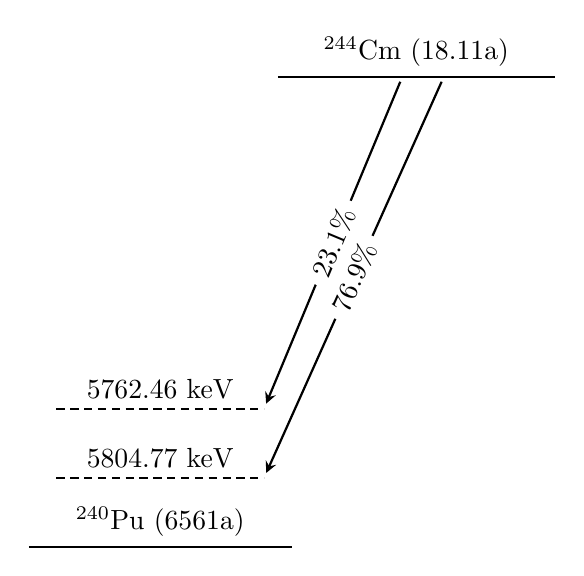
\begin{tikzpicture}[
      scale=0.5,
      level/.style={thick},
      virtual/.style={thick,densely dashed},
      trans/.style={thick,->,shorten >=2pt,shorten <=2pt,>=stealth},
      classical/.style={thin,double,<->,shorten >=4pt,shorten <=4pt,>=stealth}
    ]
    % Draw the energy levels.
    \draw[level] (20em,18em)   -- (40em,18em) node[midway,above] {$^{244}$Cm ($18.11$a)};
    \draw[level] (2em,-16em)  -- (21em,-16em) node[midway,above] {$^{240}$Pu ($6561$a)};
    % Draw the virtual levels.
    \draw[virtual] (4em,-6em)  -- (19em,-6em)  node[midway,above] {5762.46 keV};
    \draw[virtual] (4em,-11em)  -- (19em,-11em)  node[midway,above] {5804.77 keV};
    %    \draw[virtual] (0cm,-11em) -- (4cm,-11em) node[midway,above] {5.155 MeV};
    % Draw the transitions.
    \draw[trans] (29em, 18em) -- node[sloped,fill=white] {$23.1\%$} (19em, -6em);
    \draw[trans] (32em, 18em) -- node[sloped,fill=white] {$76.9\%$} (19em, -11em);
    %    \draw[classical] (4.5cm,-8em) -- (1.5cm,-5em) node[midway,below] {\Ga{}};
    \end{tikzpicture}
  }
%}
%\caption{Zerfallsschema}
%\end{figure}


%  Authors: BALRAJ SINGH, E. BROWNE   Citation:Nuclear Data Sheets 109,
%  2439 (2008)
%  
%  http://www.nndc.bnl.gov/nudat2/decaysearchdirect.jsp?nuc=244CM&unc=nds
%  
%  Half-Life: 18.11a
%  
%  Alphas:
%  
%  Energy 
%  (keV)	Intensity 
%  (%)	Dose 
%  ( MeV/Bq-s )
%    4920 3 	     5.0E-5 % 5 	  2.46E-6 25 
%    4960 3 	     1.49E-4 % 16 	  7.4E-6 8 
%    5166.64 7 	     4E-6 % 3 	  2.1E-7 15 
%    5215 3 	     5.6E-5 % 5 	  2.9E-6 3 
%    5315	     4E-5 %	  2.126E-6
%    5513 3 	     0.00352 % 18 	  1.94E-4 10 
%    5664 3 	     0.0204 % 15 	  0.00116 8 
%  *  5762.64 3 	    23.10 % 10 	  1.331 6 
%  *  5804.77 5 	    76.90 % 10 	  4.464 6 
%  

